\hsection{Weak Entities}%
%
\begin{figure}%
\centering%
%
\subfloat[][%
A reproduction of \cref{fig:erdPerson4} from back in \dref{sec:conceptual:relationshipCardinalities}, which was created using \yEd.%
\label{fig:erdPerson4B}%
]{\includegraphics[width=0.97\linewidth]{\figErdPersonIV}}%
%
\floatRowSep%
%
\subfloat[][%
A transformation of \cref{fig:erdPerson4} to a logical model using \pgmodeler.%
\label{fig:logicalErdPerson4}%
]{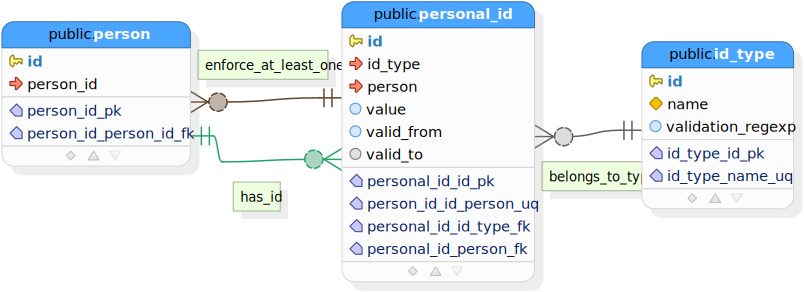
\includegraphics[width=0.9\linewidth]{\currentDir/logicalErdPerson4}}%
%
\caption{The representation of weak entities as tables bound with mandatory relationships.}%
\label{fig:logicalErdPerson4X}%
\end{figure}%
%
As introduced in \cref{sec:weakEntities}, weak entity types always appear in at least one identifying relationship with a strong entity type~\cite{S2024D:MEDTRDM}.
In \cref{fig:erdPerson4} back in \dref{sec:conceptual:relationshipCardinalities}, which is here reprinted as \cref{fig:erdPerson4B}, we modeled IDs that belong to a person as such a week entity type.
Each \emph{Personal~ID} is in an identifying relationship with an entity of type~\emph{Person} and also in an identifying relationship with an entity of type~\emph{ID~Type}.

If we map such identifying relationships to \sql, then they must be represented with mandatory ends on the sides opposing the weak entity type.
In other words, the relationships must be such that they enforce that the weak entity is connected to the strong entities.
This is
If we look at \cref{fig:erdPerson4B}, then this would mean that we need to model the following two relationships:%
%
\begin{itemize}%
\item \crowsFoot{Person}{M1}{Personal~ID}{MM}, which we can do based on \cref{sec:rm:mn} and%
\item \crowsFoot{Personal~ID}{OM}{ID~Type}{M1}, i.e., \crowsFoot{ID~Type}{M1}{Personal~ID}{OM}, which we can do based on \cref{sec:rm:kl}.%
\end{itemize}%
%
For the modeling, we will this time use the \pgmodeler.
We will basically have to enter the same constraints and table formats as we would do via \sql, but can use a  more convenient \pgls{GUI}.
The transformation of \cref{fig:erdPerson4B} to the logical model via \pgmodeler\ is illustrated in \cref{fig:logicalErdPerson4}.%
%
\begin{sloppypar}%
Back in \cref{sec:rm:mn}, we needed \emph{two} foreign key \sqlil{REFERENCES} constraints to enforce the \crowsFoot{M}{M1}{N}{MM}.
On the one hand, we referenced table~\sqlil{M} from table~\sqlil{N} with a single foreign key that was~\sqlil{NOT NULL}.
This enforced that there was at least one row in table~\sqlil{M} for each row in table~\sqlil{N}.
On the other hand, we referenced table~\sqlil{N} from table~\sqlil{M} with a compound foreign key.
This enforced that each one row in table~\sqlil{M} was connected to one row in table~\sqlil{N}, while not preventing that more rows in table~\sqlil{N} may exist that are related to it.%
\end{sloppypar}%
%
If we enter the same constraints into \pgmodeler, it will display them separately.
Indeed, this offers another perspective on the way we modeled the \crowsFoot{M}{M1}{N}{MM} relationship in \sql:
Actually, we did realize it as a combination of a \crowsFoot{M}{O1}{N}{M1} and a \crowsFoot{M}{M1}{N}{OM} relationship.%
%
\begin{itemize}\sloppy%
%
\item The brown \crowsFoot{\sqlil{person}}{OM}{\sqlil{personal_id}}{M1} relationship called \emph{enforce\_at\_least\_one} in \cref{fig:logicalErdPerson4} uses a composite foreign key and makes sure that, for each row in table~\sqlil{person}, at least one related row in table~\sqlil{personal_id} exists.
It will be imposed to table~\sqlil{person}.%
%
\item The green \crowsFoot{\sqlil{person}}{M1}{\sqlil{personal_id}}{OM} relationship called \emph{has\_id} in \cref{fig:logicalErdPerson4} uses a single foreign key in table~\sqlil{personal_id} and enforces that each row in that table is related to exactly one row in table~\sqlil{person}.%
It is imposed on table~\sqlil{personal_id}.%
%
\end{itemize}\fussy%
%
\begin{figure}%
\centering%
%
\subfloat[][%
In the \pgmodeler\ design view, right-click and select \menu{New > Schema Object > Sequence}.%
\label{fig:pgmodelerSequence1new}%
]{\tightbox{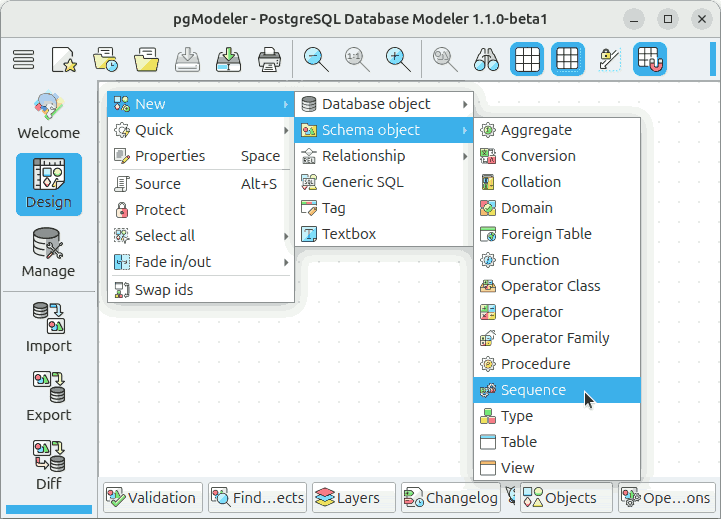
\includegraphics[width=0.47\linewidth]{\currentDir/pgmodelerSequence1new}}}%
%
\floatSep%
%
\subfloat[][%
In the dialog that pops up, we first enter a reasonable name for our \sqlilIdx{SEQUENCE}. %
Here we choose \sqlil{person_id_counter}. %
Then we click~\menu{Apply}.%
\label{fig:pgmodelerSequence2apply}%
]{\tightbox{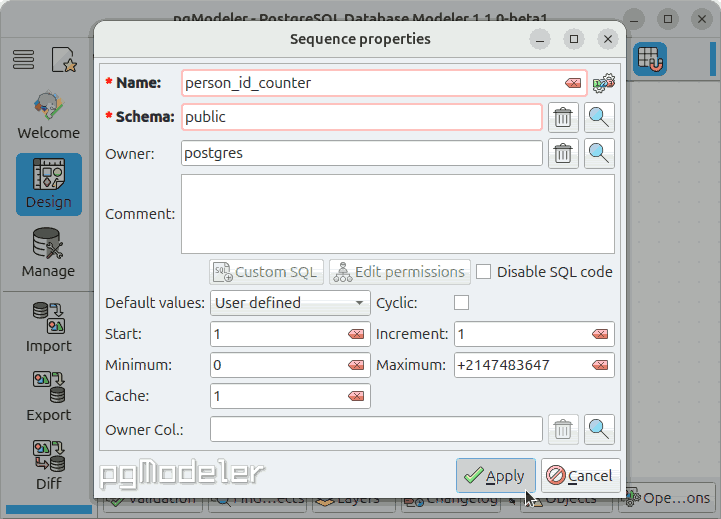
\includegraphics[width=0.47\linewidth]{\currentDir/pgmodelerSequence2apply}}}%
%
\floatRowSep%
%
\subfloat[][%
Later, when adding columns to a table, we can use the sequence. %
We select \emph{Sequence} as \menu{Default Value} and then click into the text box to the right of \emph{Sequence}.%
\label{fig:pgmodelerSequence3sequence}%
]{\tightbox{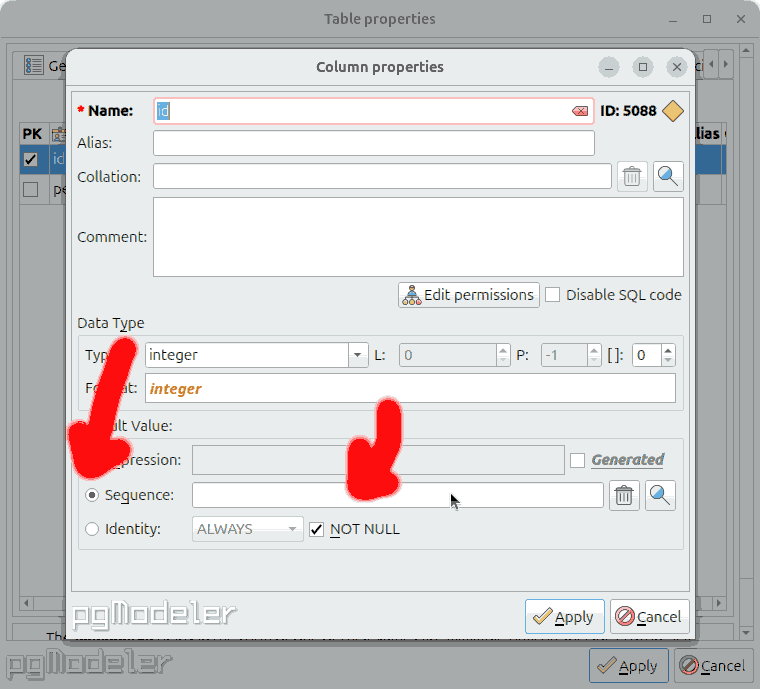
\includegraphics[width=0.47\linewidth]{\currentDir/pgmodelerSequence3sequence}}}%
%
\floatSep%
%
\subfloat[][%
Another dialog opens up where we click through the tree of objects, find our new \sqlil{Sequence}, and then click the check mark button at the bottom.%
\label{fig:pgmodelerSequence4selectSequence}%
]{\tightbox{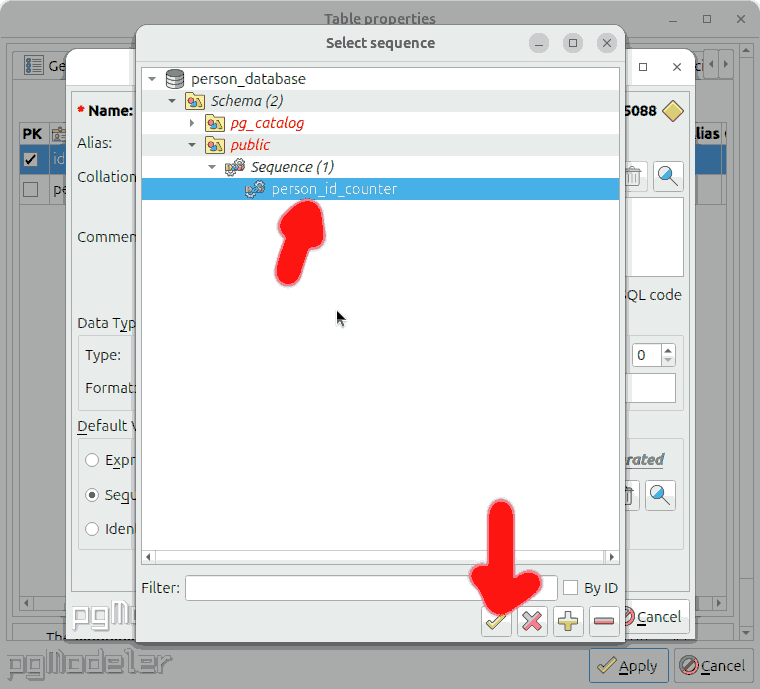
\includegraphics[width=0.47\linewidth]{\currentDir/pgmodelerSequence4selectSequence}}}%
\floatRowSep%
%
\subfloat[][%
The sequence is now selected and the column will take its default values from it.%
\label{fig:pgmodelerSequence5selected}%
]{\tightbox{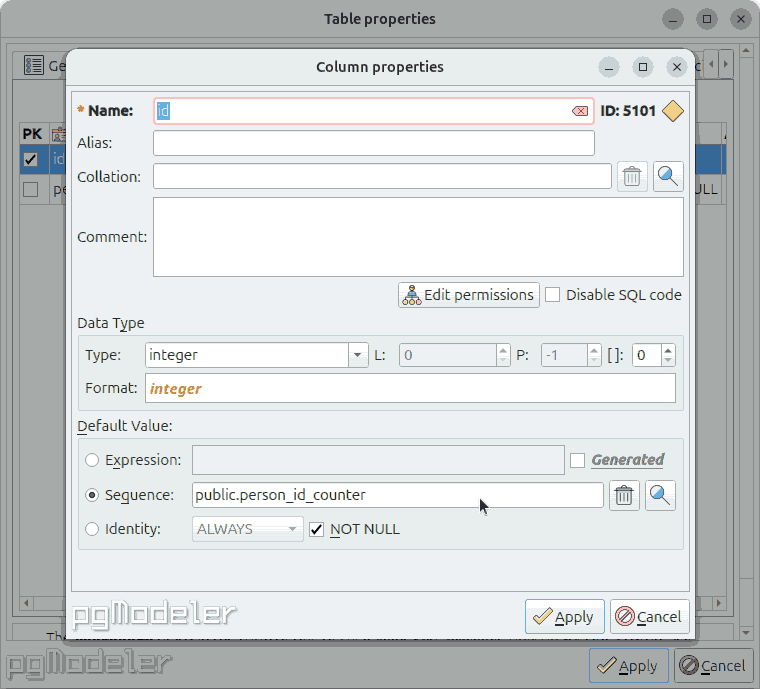
\includegraphics[width=0.5\linewidth]{\currentDir/pgmodelerSequence5selected}}}%
%
\caption{Using the \sqlilIdx{SEQUENCE} feature in \pgmodeler.}%%
\label{fig:pgmodelerSequence}%
\end{figure}%

Notice that we used the \sqlilIdx{SEQUENCE} feature when creating the model for the \crowsFoot{M}{M1}{N}{MM} setup in \cref{sec:rm:mn}.
While I will not go into detail on how we create the whole logical model, let us briefly discuss how to use this feature in \pgmodeler.
It is rather easy.
We begin by opening the \pgmodeler\ in the design view.
We right-click into the workspace and select \menu{New > Schema Object > Sequence}, as shown in \cref{fig:pgmodelerSequence1new}.

In the dialog that pops up, we first enter a reasonable name for our \sqlilIdx{SEQUENCE}.
Here we choose \sqlil{person_id_counter}, because we will use the sequence to generate the values for the \sqlil{id} column of the \sqlil{person} table.
Then we click~\menu{Apply}, as sketched in \cref{fig:pgmodelerSequence2apply}.

Later, when adding columns to a table~\sqlil{person}, we can use the sequence.
We therefore select \emph{Sequence} as \menu{Default Value}.
In \cref{fig:pgmodelerSequence3sequence}, we then click into the text box to the right of \emph{Sequence}.
As illustrated in \cref{fig:pgmodelerSequence4selectSequence}, another dialog opens up where we click through the tree of objects, find our new \sqlil{Sequence}, and then click the check mark button at the bottom.
In \cref{fig:pgmodelerSequence5selected}, the sequence is now selected and the column will take its default values from it.

\gitLoadAndExecSQL{person_1:01_person_database_database_2001}{}{teachingManagement/logical/person_database_1/generated_sql}{01_person_database_database_2001.sql}{}{}{}%
\listingSQL{person_1:01_person_database_database_2001}{%
The generated script to create the \sqlil{person_database}~\db.}%
%
\gitLoadAndExecSQL{person_1:03_public_person_id_counter_sequence_5071}{}{teachingManagement/logical/person_database_1/generated_sql}{03_public_person_id_counter_sequence_5071.sql}{person_database}{}{}%
\listingSQL{person_1:03_public_person_id_counter_sequence_5071}{The generated script to create ID~\sqlilIdx{SEQUENCE}.}%
%
\gitLoadAndExecSQL{person_1:04_public_id_type_table_5072}{}{teachingManagement/logical/person_database_1/generated_sql}{04_public_id_type_table_5072.sql}{person_database}{}{}%
\listingSQL{person_1:04_public_id_type_table_5072}{The generated script to create the \sqlil{id_type} table.}%
%
\gitLoadAndExecSQL{person_1:05_public_personal_id_table_5078}{}{teachingManagement/logical/person_database_1/generated_sql}{05_public_personal_id_table_5078.sql}{person_database}{}{}%
\listingSQL{person_1:05_public_personal_id_table_5078}{The generated script to create the \sqlil{personal_id} table.}%
%
\gitLoadAndExecSQL{person_1:06_public_person_table_5087}{}{teachingManagement/logical/person_database_1/generated_sql}{06_public_person_table_5087.sql}{person_database}{}{}%
\listingSQL{person_1:06_public_person_table_5087}{The generated script to create the \sqlil{personal_id} table.}%
%
\gitLoadAndExecSQL{person_1:07_public_personal_id_personal_id_id_type_fk_constraint_5093}{}{teachingManagement/logical/person_database_1/generated_sql}{07_public_personal_id_personal_id_id_type_fk_constraint_5093.sql}{person_database}{}{}%
\listingSQL{person_1:07_public_personal_id_personal_id_id_type_fk_constraint_5093}{The generated script to create the constraint managing the relationship between the rows in table~\sqlil{personal_id} and those in table~\sqlil{id_type}.}%
%
\gitLoadAndExecSQL{person_1:08_public_personal_id_personal_id_person_fk_constraint_5094}{}{teachingManagement/logical/person_database_1/generated_sql}{08_public_personal_id_personal_id_person_fk_constraint_5094.sql}{person_database}{}{}%
\listingSQL{person_1:08_public_personal_id_personal_id_person_fk_constraint_5094}{The generated script to create the constraint that enforces that each row in table~\sqlil{personal_id} is related to exactly one row in table~\sqlil{person}.}%
%
\gitLoadAndExecSQL{person_1:09_public_person_person_id_person_id_fk_constraint_5092}{}{teachingManagement/logical/person_database_1/generated_sql}{09_public_person_person_id_person_id_fk_constraint_5092.sql}{person_database}{}{}%
\listingSQL{person_1:09_public_person_person_id_person_id_fk_constraint_5092}{The generated script to create the constraint that enforces that, for each row in table~\sqlil{person}, at least one related row in table~\sqlil{personal_id} exists.}%
%
\gitLoadAndExecSQL{person_database_1:insert_and_select}{}{teachingManagement/logical/person_database_1}{insert_and_select.sql}{person_database}{}{}%
\listingSQLandOutput{person_database_1:insert_and_select}{insert_and_select.sql}{%
Inserting into and selecting data from the tables in the \sqlil{person_database}.%
}{}%
%
\gitExecSQLraw{}{}{teachingManagement/logical/person_database_1}{cleanup.sql}{}{}{}%
%
\Cref{lst:person_1:01_person_database_database_2001,lst:person_1:03_public_person_id_counter_sequence_5071,lst:person_1:04_public_id_type_table_5072,lst:person_1:05_public_personal_id_table_5078,lst:person_1:06_public_person_table_5087,lst:person_1:07_public_personal_id_personal_id_id_type_fk_constraint_5093,lst:person_1:08_public_personal_id_personal_id_person_fk_constraint_5094,lst:person_1:09_public_person_person_id_person_id_fk_constraint_5092} illustrate the generated \sql\ scripts corresponding to this logical model.
In \cref{lst:person_1:01_person_database_database_2001}, the empty new \db\ \sqlil{person_database} is created.
\Cref{lst:person_1:03_public_person_id_counter_sequence_5071} creates the sequence that we will use to generate the primary keys~\sqlil{id} of the \sqlil{person} table.

\Cref{lst:person_1:04_public_id_type_table_5072} creates the table for the ID~types.
This table has the primary key~\sqlil{id} and an attribute~\sqlil{name}, which must be \sqlilIdx{UNIQUE}.
It also has a column \sqlil{validation_regex} in which we will store a \pgls{regex} that applications can use to validate the input for a given ID~type.
This column must be~\sqlilIdx{NOT NULL} and has the default value~\sqlil{'.+'}, which is the \pgls{regex} for \inQuotes{at least one character}.
In other words, unless the \pgls{dba} provides a better \pgls{regex}, applications are told to check that an ID always consists of at least one character.

\Cref{lst:person_1:05_public_personal_id_table_5078} creates that table in which we will store the \emph{Personal ID} entities.
Like all of our tables, it has a surrogate primary key~\sqlil{id}.
The \emph{Personal~ID} entities are weak entities.
They cannot exist without a defining relationship to one \emph{Person} entity and one \emph{ID~Type} entity.
Therefore, this table stores two foreign keys:
\sqlil{id_type} and \sqlil{person}.
The corresponding constraints are added later in \cref{lst:person_1:07_public_personal_id_personal_id_id_type_fk_constraint_5093,lst:person_1:08_public_personal_id_personal_id_person_fk_constraint_5094}, respectively.
The table has a \sqlilIdx{UNIQUE} constraint imposed on the tuples of the surrogate key~\sqlil{id} and the foreign key~\sqlil{person}, because later, the table~\sqlil{person} will use this tuple as composite foreign key.

In \cref{lst:person_1:06_public_person_table_5087}, the table~\sqlil{person} is created.
In this part of our example, we do not model much additional information about the \emph{Person} entities.
Therefore, this table only has a surrogate primary key~\sqlil{id}.
However, we imposed the requirement that our system must have stored some form of identification for each entity of type~\emph{Person}.
Therefore, we also have the foreign key~\sqlil{person_id} pointing to the table~\sqlil{personal_id} with the weak \emph{Personal ID} entities.
From our treatment of the \crowsFoot{M}{M1}{N}{MM} relationship pattern in \cref{sec:rm:mn}, we know that this table must use a composition foreign key, which is created in \cref{lst:person_1:09_public_person_person_id_person_id_fk_constraint_5092}.
This key makes sure that each row in table~\sqlil{person} has at least one corresponding row in table~\sqlil{personal_id}.

We create all the tables by executing all of the above scripts.
Then, we can insert data into them by writing and running our own \sql\ script.
Such a script is illustrated in \cref{lst:person_database_1:insert_and_select}.
We start out by inserting two rows into the table~\sqlil{id_type}, one for Chinese ID numbers~(中国公民身份号码) and one for Chinese mobile phone numbers.
We store the same \pglspl{regex} that we used in \cref{sec:mappingEntitiesToTables}.
Of course, now, we are only working on a part of a logical model of the teaching management system.
So there is no application that actually uses these \pglspl{regex}.
But at least in our imagination, we would have provided the means for checking ID values.

Then we use basically the same code as in \cref{lst:MN_insert_and_select} from back in \dref{sec:rm:mn} to fill the tables~\sqlil{person} and \sqlil{personal_id}.
First we create a \sqlil{person} record with an associated Chinese national~ID, then we add a mobile phone number to that record.
Then we create a second record, again with national~ID.
At the end, we combine the information back together using an~\sqlilIdx{INNER JOIN}.

One may ask whether it is really useful to go through the hassle to enforce that each \emph{Person} entity does have at least one associated~\emph{Personal ID}~entity.
This is a valid question.
Creating the proper constraints to fully represent the logical relationship imposed by the conceptual model and the weak entity structure requires considerable effort.
It also forces us to use the \sqlilIdx{SEQUENCE} feature, which is not supported by some \pglspl{dbms}, and the \sqlilIdx{RETURNING}~feature, which is also not supported by several systems.

It thus may be much easier to choose a \crowsFoot{Person}{M1}{Personal~ID}{OM} relationship structure instead of the \crowsFoot{Person}{M1}{Personal~ID}{MM} pattern.
Doing this would allow us to remain in the realm of plain and simple standard~\sql.
We would have to trust the person tasked with entering data about students and faculty members that they will always require and properly enter some form of~ID, even if the underlying \db\ would permit ID\nobreakdashes-less entries.
We would not apply follow our conceptual model exactly.
We would also reduce our \inQuotes{defense in depth} approach from \cref{bp:defenseInDepth}, which emphasizes on using as many constraints and sanity checks as possible in all layers of our application.
But we would get much simpler code, which is easier to check and easier to maintain.
Also, if an application would later enter data, maybe via a library like \psycopg, the complexity of the required access pattern would also be reduced.
What to do here is a an interesting philosophical question, with no clear right or wrong choice.

In this book, we choose the harder method {\dots} just to see whether we can get it to work.
Anyway, after running this example we delete the \sqlil{person_database} with a \sqlilIdx{DROP DATABASE} command.
%
\FloatBarrier%
\endhsection%
%
